
The script that solves the problem is \ttt{laplace.m} and is available at the end of the report with the subroutine \ttt{sol.m}. The boundary conditions in equation~\eqref{eq:cond2} are treated with ghost points. The conditions that the ghost point has the same value as the last point in the \textit{interior} of the domain. This is given by the discrete first derivative set to zero. We have numbered our unknowns vertically on the grid so that the band size is $M+2$ which is smaller than $N$ (the band we obtain when numbering the unknowns horizontally).

Here is the output of our script. With figures~\ref{fig:h02} and~\ref{fig:h01}.

\begin{lstlisting}
>> laplace
T(2,1) = 450.0000000000003979 for h = 0.2 
T(2,1) = 449.9999999999993747 for h = 0.1 
\end{lstlisting}

\begin{figure}[!h]
\centering
\includegraphics[width = 0.7\textwidth]{./h02.eps}
\caption{Solution with matlab for $h = 0.2$}
\label{fig:h02}
\end{figure}

\begin{figure}[!h]
\centering
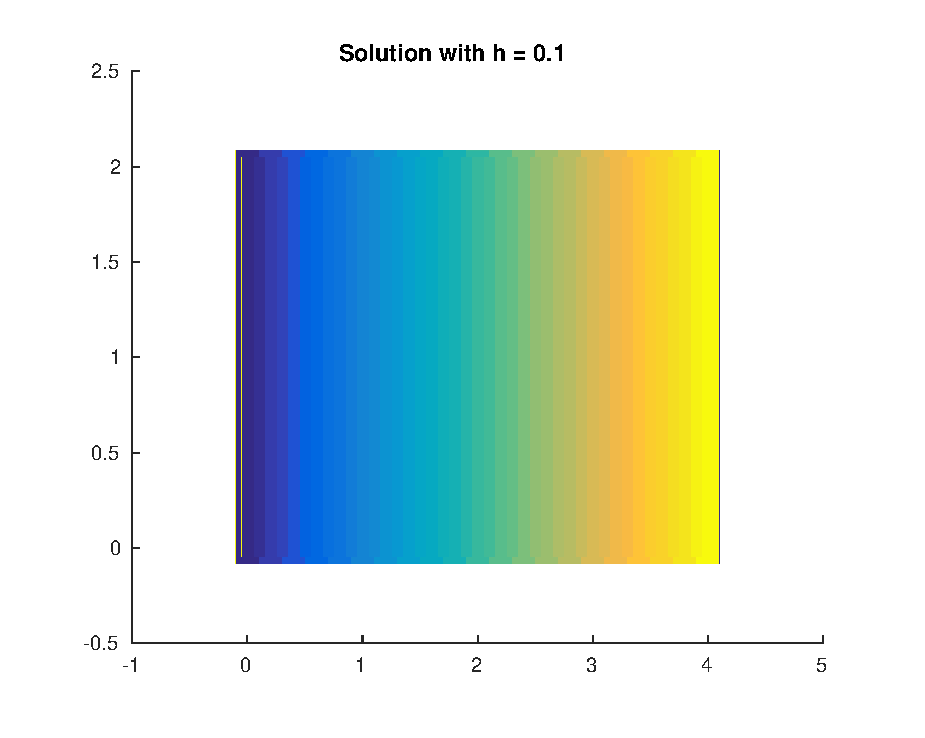
\includegraphics[width = 0.7\textwidth]{./h01.eps}
\caption{Solution with matlab for $h = 0.1$}
\label{fig:h01}
\end{figure}

\FloatBarrier

We see that the exact value at $(2,1)$ is close to $450$. It is clear by symmetry that the solution does not depend en the y-coordinate. Therefore the equation reduces to $$\dfrac{\dr^{2} T}{\dr x^{2}}=0.$$
The solution is a plane $$T(x,y)=T(x)= ax+b.$$ 
The boundary conditions $T(x=0)=300$ and $T(x=4)=600$ allow to find that $T(x)= 300+ 75x$. The solution respects boundary conditions~\eqref{eq:cond1} and~\eqref{eq:cond2}. It is now clear that $T(2,1)=450$. The (notably small) errors in the numerical solution are \textit{only} due to floating point computation errors. 
